
\chapter{Grid Page}
The first page you will be presented with after loading or creating a new project is the Grid Page. This is the main page of MCL and is used to access the firmware's sub-pages and menus.

\begin{center}
	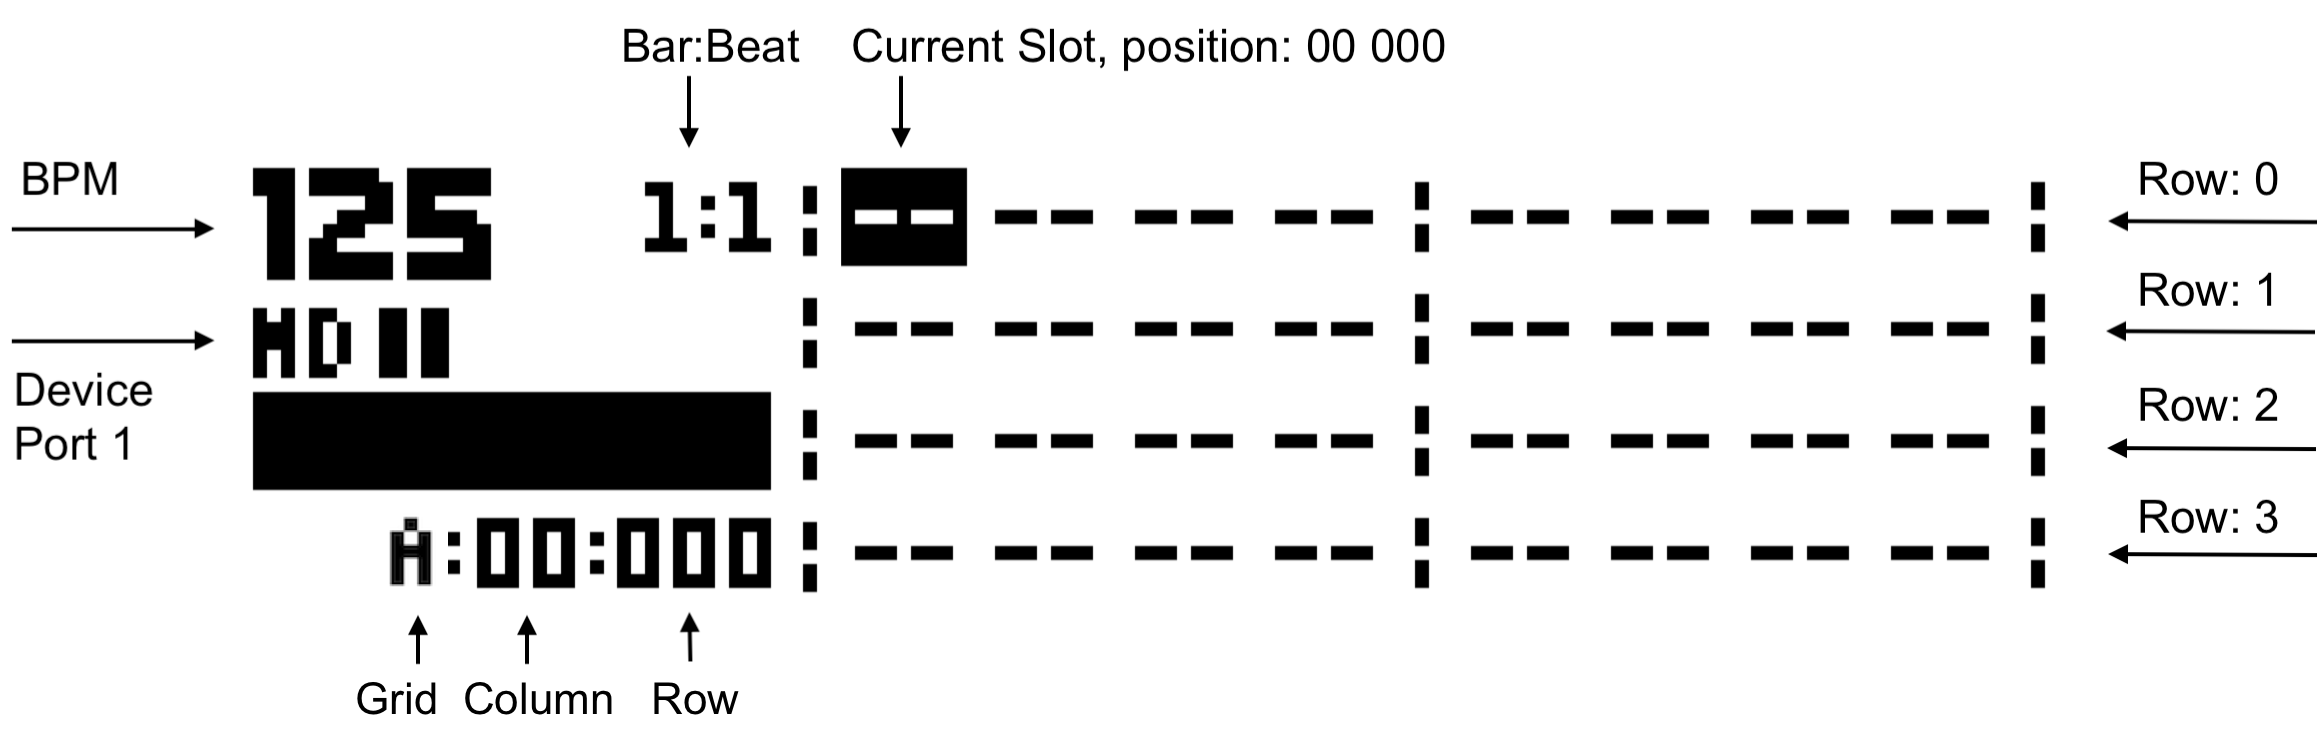
\includegraphics[scale=.40]{grid_init_annot.png}
\end{center}
MCL displays the Grid on screen. Four rows are drawn on screen at any one time with each row showing 8 out of 20 slots.\\
\\
Occupied slots will show the Machine Type associated with the track for example "BD" for Bass Drum. Unoccupied Slots are represented by two lines of "--" . For clarity, a dashed vertical line is printed after every fourth slot. \\
\\
The current slot's column and row are displayed towards the bottom left of the screen.\\
\\
An interactive cursor indicates the current slot position and is distinguished by a slot printed with inverted colours.
\section{Encoder Assignment:}
Rotating encoders 1 or 2 will allow the current slot position to change.\\
\\
When the cursor reaches the edges of the screen you can continue to scroll through the grid:
\begin{itemize}
	\item \textbf{[Encoder 1]:} scrolls the grid horizontally.
	\item \textbf{[Encoder 2]:} scrolls the grid vertically.
	\item \textbf{[Encoder 3]:} --
	\item \textbf{[Encoder 4]:} --
\end{itemize}


